\documentclass{article}
\usepackage[margin=2cm]{geometry}
\usepackage{tikz}
\usetikzlibrary{shapes.geometric, arrows.meta, positioning}

% Define flowchart styles
\tikzstyle{startstop} = [
    rectangle, 
    rounded corners, 
    minimum width=3cm, 
    minimum height=1cm,
    text centered, 
    draw=black, 
    fill=red!30,
    font=\bfseries
]

\tikzstyle{io} = [
    trapezium, 
    trapezium left angle=70, 
    trapezium right angle=110, 
    minimum width=3cm, 
    minimum height=1cm, 
    text centered, 
    draw=black, 
    fill=blue!30
]

\tikzstyle{process} = [
    rectangle, 
    minimum width=3cm, 
    minimum height=1cm, 
    text centered, 
    draw=black, 
    fill=orange!30
]

\tikzstyle{decision} = [
    diamond, 
    minimum width=3cm, 
    minimum height=1cm, 
    text centered, 
    draw=black, 
    fill=green!30,
    aspect=2
]

\tikzstyle{arrow} = [thick,->,>=Stealth]

\title{Algorithm Flowcharts - Topic 2}
\author{Attendance Recognition Project}
\date{\today}

\begin{document}

\maketitle

\section{Algorithm 1: Even/Odd Number Checker}

This flowchart demonstrates a simple decision algorithm that determines whether a number is even or odd.

\begin{center}
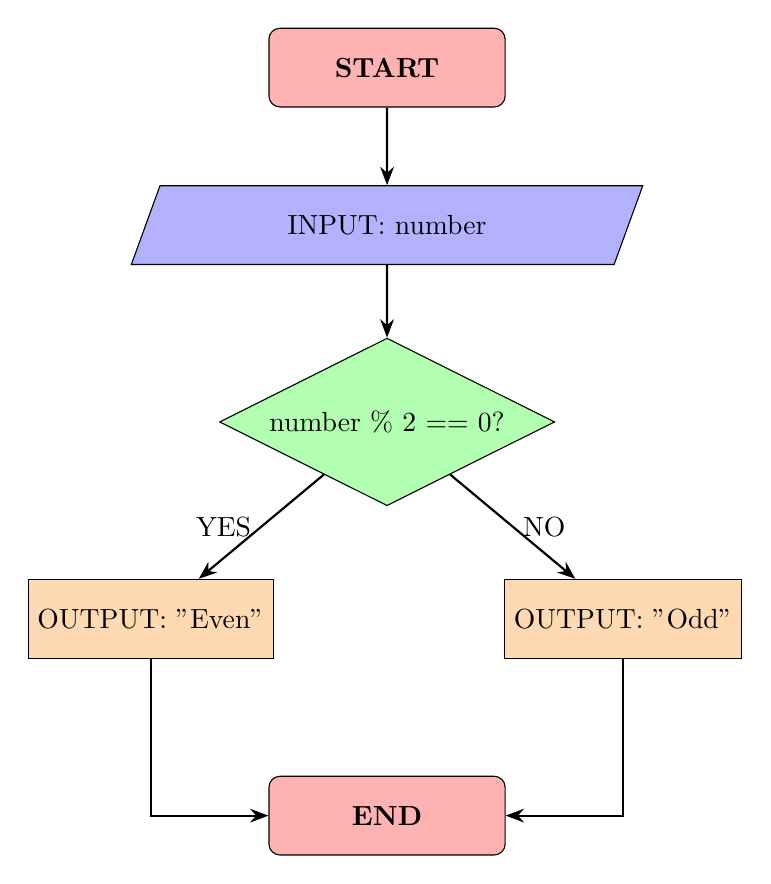
\begin{tikzpicture}[node distance=2cm]

% Nodes
\node (start) [startstop] {START};
\node (input) [io, below of=start] {INPUT: number};
\node (decision) [decision, below of=input, yshift=-0.5cm] {number \% 2 == 0?};
\node (even) [process, below of=decision, xshift=-3cm, yshift=-0.5cm] {OUTPUT: "Even"};
\node (odd) [process, below of=decision, xshift=3cm, yshift=-0.5cm] {OUTPUT: "Odd"};
\node (end) [startstop, below of=decision, yshift=-3cm] {END};

% Arrows
\draw [arrow] (start) -- (input);
\draw [arrow] (input) -- (decision);
\draw [arrow] (decision) -- node[anchor=east] {YES} (even);
\draw [arrow] (decision) -- node[anchor=west] {NO} (odd);
\draw [arrow] (even) |- (end);
\draw [arrow] (odd) |- (end);

\end{tikzpicture}
\end{center}

\textbf{Algorithm Description:}
\begin{enumerate}
    \item Start the program
    \item Read input number from user
    \item Check if number modulo 2 equals 0
    \item If YES: Display "Even"
    \item If NO: Display "Odd"
    \item End the program
\end{enumerate}

\newpage

\section{Algorithm 2: Factorial Calculator}

This flowchart shows a loop-based algorithm for calculating the factorial of a number.

\begin{center}
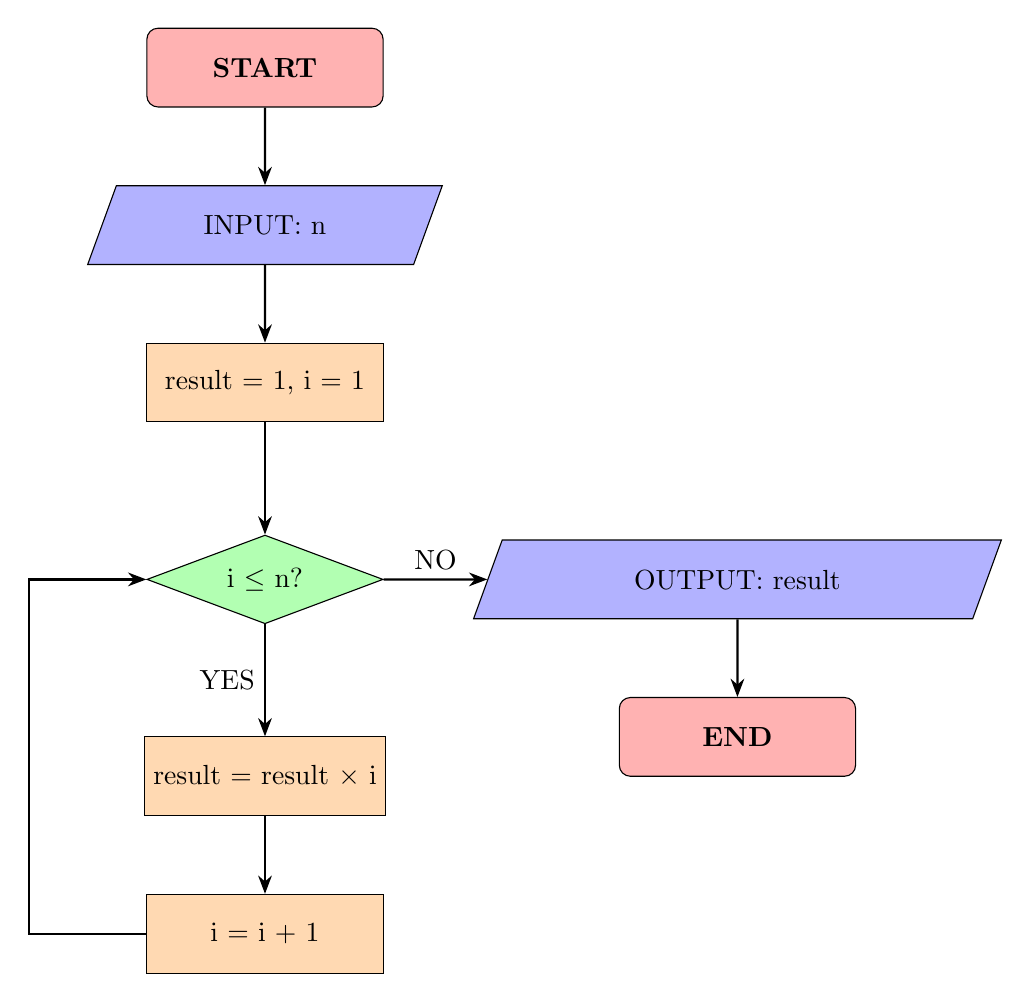
\begin{tikzpicture}[node distance=2cm]

% Nodes
\node (start) [startstop] {START};
\node (input) [io, below of=start] {INPUT: n};
\node (init) [process, below of=input] {result = 1, i = 1};
\node (decision) [decision, below of=init, yshift=-0.5cm] {i \(\leq\) n?};
\node (multiply) [process, below of=decision, yshift=-0.5cm] {result = result \(\times\) i};
\node (increment) [process, below of=multiply] {i = i + 1};
\node (output) [io, right of=decision, xshift=4cm] {OUTPUT: result};
\node (end) [startstop, below of=output] {END};

% Arrows
\draw [arrow] (start) -- (input);
\draw [arrow] (input) -- (init);
\draw [arrow] (init) -- (decision);
\draw [arrow] (decision) -- node[anchor=east] {YES} (multiply);
\draw [arrow] (multiply) -- (increment);
\draw [arrow] (increment) -- +(-3,0) |- (decision);
\draw [arrow] (decision) -- node[anchor=south] {NO} (output);
\draw [arrow] (output) -- (end);

\end{tikzpicture}
\end{center}

\textbf{Algorithm Description:}
\begin{enumerate}
    \item Start the program
    \item Read input number n from user
    \item Initialize result = 1 and counter i = 1
    \item Check if i \(\leq\) n
    \item If YES:
    \begin{itemize}
        \item Multiply result by i
        \item Increment i by 1
        \item Go back to step 4
    \end{itemize}
    \item If NO: Display result
    \item End the program
\end{enumerate}

\textbf{Example:} For n = 5:
\begin{itemize}
    \item i=1: result = 1 \(\times\) 1 = 1
    \item i=2: result = 1 \(\times\) 2 = 2
    \item i=3: result = 2 \(\times\) 3 = 6
    \item i=4: result = 6 \(\times\) 4 = 24
    \item i=5: result = 24 \(\times\) 5 = 120
    \item i=6 > 5: Output 120
\end{itemize}

\section{Flowchart Symbols Reference}

\begin{center}
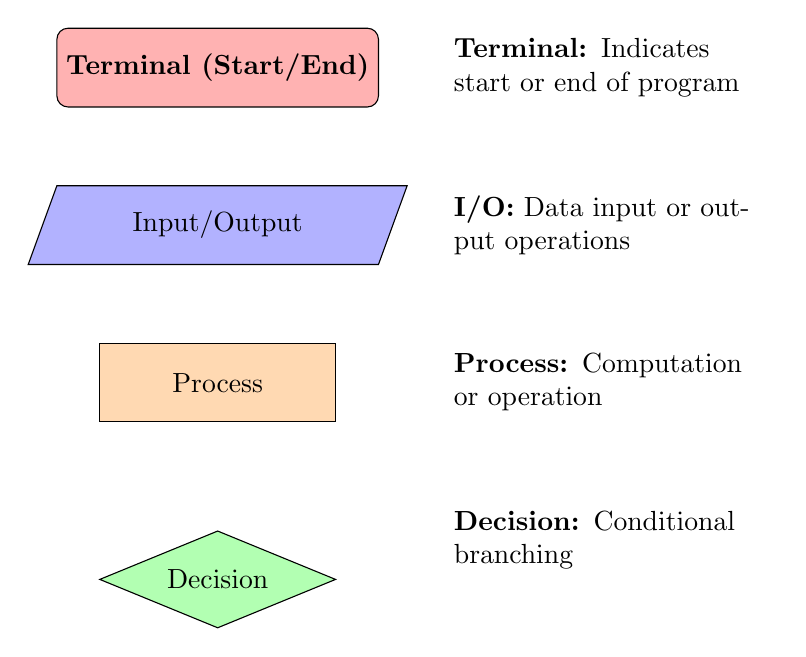
\begin{tikzpicture}[node distance=3cm]

\node (term) [startstop] {Terminal (Start/End)};
\node (io) [io, below of=term, yshift=1cm] {Input/Output};
\node (proc) [process, below of=io, yshift=1cm] {Process};
\node (dec) [decision, below of=proc, yshift=0.5cm] {Decision};

\node[right of=term, xshift=2cm, text width=4cm] {\textbf{Terminal:} Indicates start or end of program};
\node[right of=io, xshift=2cm, text width=4cm] {\textbf{I/O:} Data input or output operations};
\node[right of=proc, xshift=2cm, text width=4cm] {\textbf{Process:} Computation or operation};
\node[right of=dec, xshift=2cm, text width=4cm, yshift=0.5cm] {\textbf{Decision:} Conditional branching};

\end{tikzpicture}
\end{center}

\end{document}
